\chapter{Sprint 5 : Visioconférence Intégrée et Gestion des Agendas} 
\minitoc
\newpage

\section{Introduction}
Bien que la messagerie instantanée asynchrone (développée lors du Sprint 3) assure un contact continu, la relation coach-athlète atteint sa plénitude lors d'échanges directs et synchrones. Qu'il s'agisse d'un bilan mensuel de progression, d'une consultation nutritionnelle poussée, ou même d'une séance d'entraînement corrigée en temps réel à distance, la visioconférence est un outil devenu indispensable pour les professionnels de la préparation physique.

Ce cinquième et dernier sprint fonctionnel aborde le défi de la communication audiovisuelle en temps réel et de l'organisation du temps de travail. Il s'agit de concevoir un module complet permettant au coach de définir ses créneaux de disponibilité sur son application Web (Angular), à l'athlète de planifier et réserver ces séances sur son application mobile (Flutter), et à ces deux acteurs d'initier une session d'appel vidéo sécurisée et fluide directement intégrée au sein de CoachingApp.

\section{Objectifs et Planification du Sprint 5}
\subsection{Backlog du Sprint 5}
Les exigences fonctionnelles retenues pour ce sprint de clôture fonctionnelle sont les suivantes :
\begin{itemize}
    \item \textbf{Tâche Backend 5.1 :} Concevoir les schémas de données PostgreSQL pour la gestion des créneaux de disponibilité (\texttt{AvailabilitySlot}) et des sessions réservées (\texttt{CoachingSession}).
    \item \textbf{Tâche Web (Angular) 5.1 :} Développer une interface d'agenda de type "Calendar View" interactive permettant au coach d'ajouter, modifier et bloquer ses plages horaires de travail hebdomadaires.
    \item \textbf{Tâche Client (Flutter) 5.1 :} Créer le module de réservation mobile permettant à l'athlète de parcourir l'agenda de son coach attitré, de sélectionner un créneau libre et de soumettre sa demande de réservation.
    \item \textbf{Tâche Fullstack 5.2 :} Intégrer la passerelle de visioconférence WebRTC sécurisée en s'interfaçant avec le SDK open-source \textbf{Jitsi Meet} afin d'instancier des salons d'appel vidéo à la volée.
\end{itemize}

\section{Conception détaillée du Sprint 5}
\subsection{Diagramme de séquence : Planification et Lancement de Visioconférence}
Le diagramme de séquence ci-dessous illustre le flux complexe d'interactions asynchrones et synchrones lors de la réservation d'un créneau et de l'accès au salon vidéo chiffré.

\begin{figure}[H]
\centering
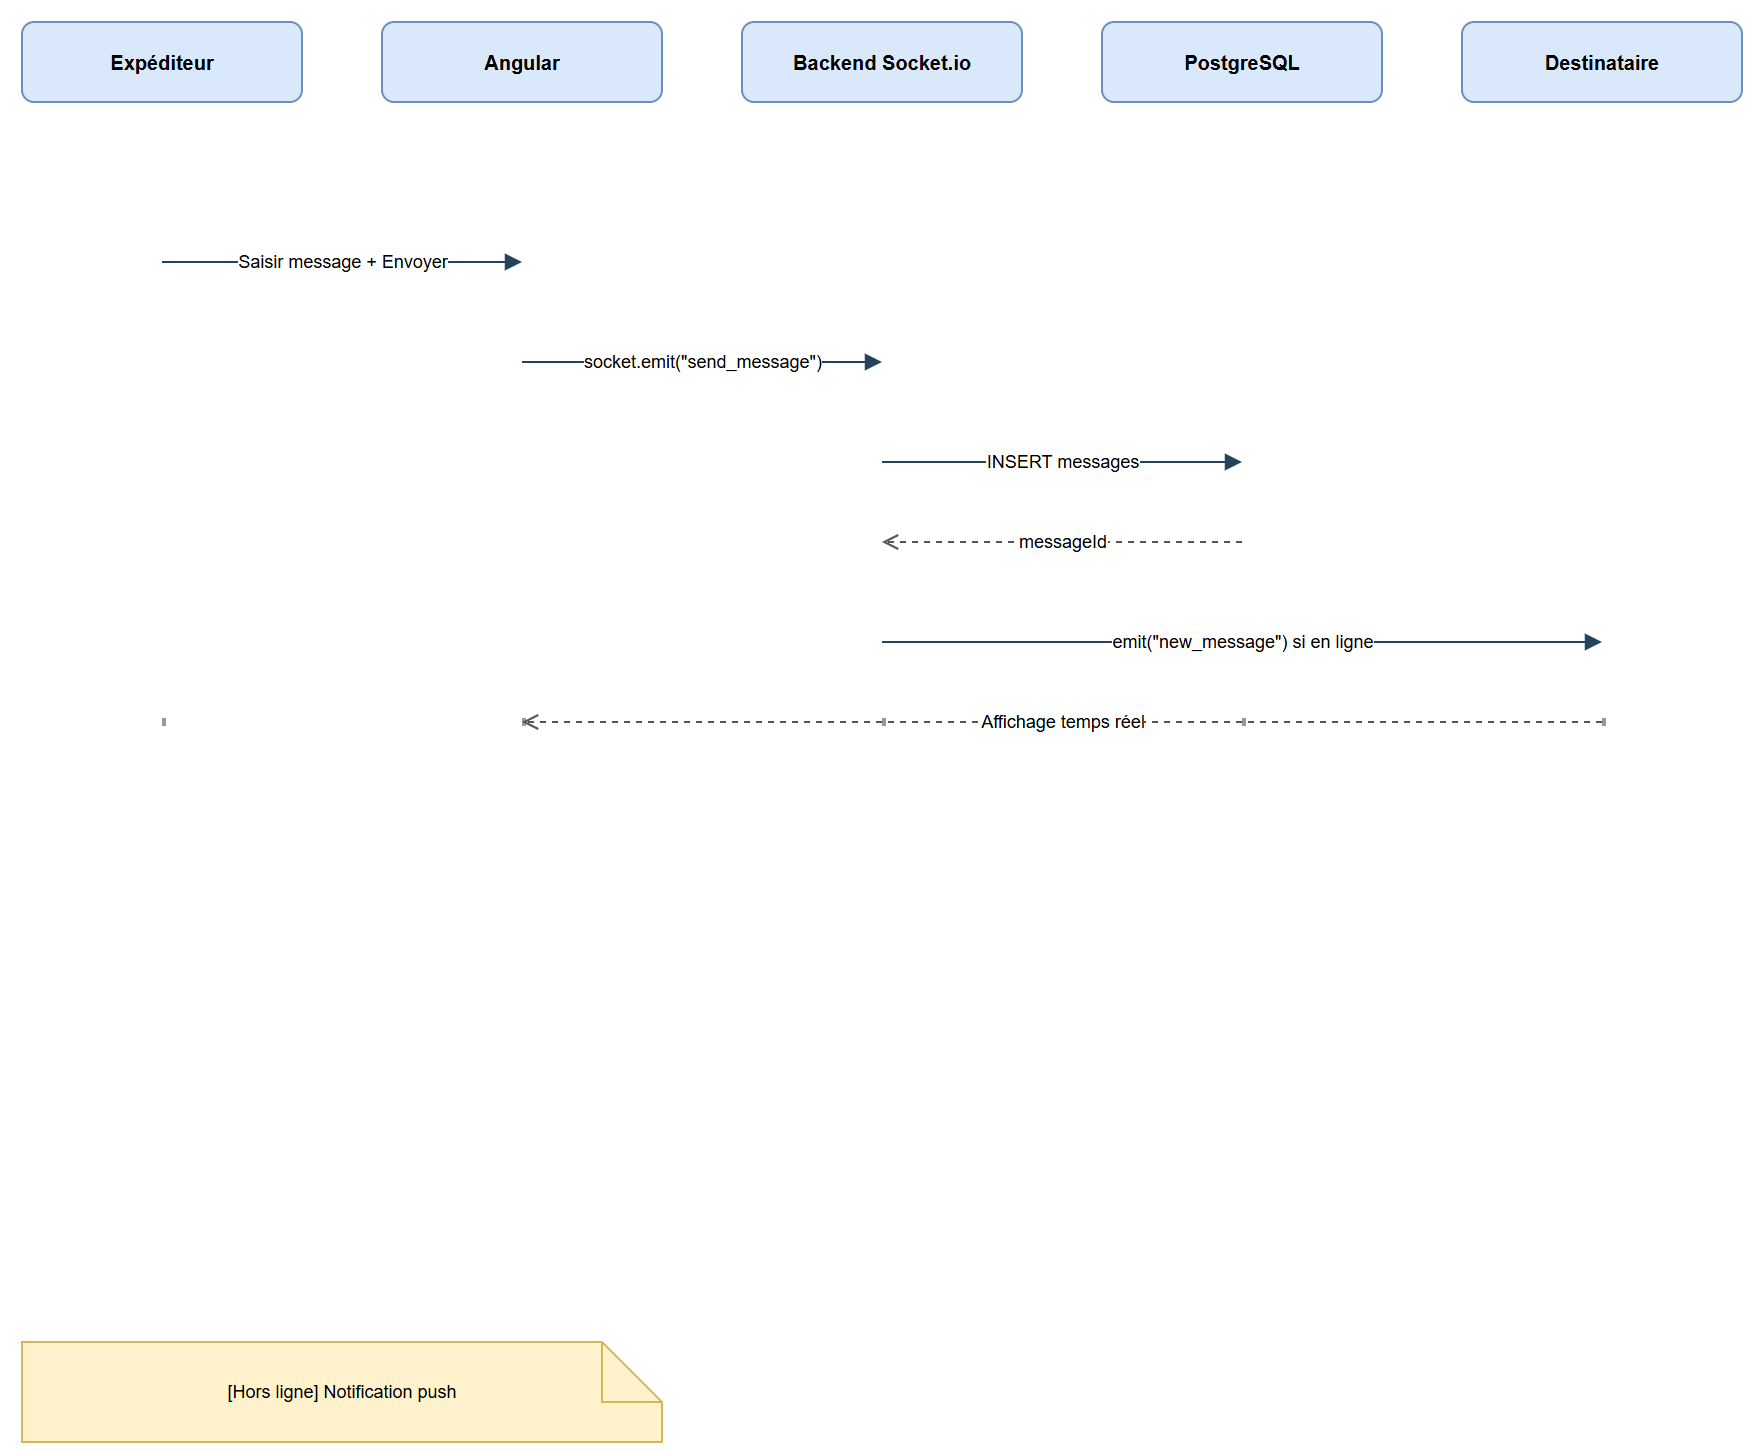
\includegraphics[width=0.9\textwidth]{diagrams/sequence sprint 5.png}
\caption{Diagramme de séquence : Réservation et Visioconférence - Sprint 5}
\end{figure}

\subsection{Modélisation Relationnelle (Base de données)}
Pour supporter ce flux, deux entités majeures ont été introduites :
\begin{itemize}
    \item \textbf{AvailabilitySlot (Créneau de disponibilité) :} Défini par une heure de début, une heure de fin et un jour de la semaine. Il appartient au coach.
    \item \textbf{CoachingSession (Session réservée) :} Matérialise le rendez-vous validé. Elle lie un \texttt{Athlete} et un \texttt{Coach}, contient un statut (\texttt{PENDING}, \texttt{CONFIRMED}, \texttt{CANCELLED}) et stocke un lien de salon unique et éphémère (\texttt{roomName}) généré cryptographiquement pour sécuriser l'accès WebRTC.
\end{itemize}

\section{Réalisation technique : La Communication Vidéo en Direct}
\subsection{Implémentation de l'Agenda Interactif (Angular)}
Côté Web, le coach gère son emploi du temps de manière très visuelle. Nous avons implémenté un service Angular gérant les appels API pour enregistrer les créneaux récurrents. L'utilisation d'Angular Reactive Forms permet de s'assurer de la cohérence des horaires (ex: l'heure de fin doit être strictement supérieure à l'heure de début).

\begin{lstlisting}[language=TypeScript, caption={Service de gestion des disponibilités côté Coach (Angular)}, label={lst:angular_availabilities}]
import { Injectable } from '@angular/core';
import { HttpClient } from '@angular/common/http';
import { Observable } from 'rxjs';
import { environment } from '../../../environments/environment';

@Injectable({
  providedIn: 'root'
})
export class AgendaService {
  private apiUrl = `${environment.apiUrl}/agenda`;

  constructor(private http: HttpClient) { }

  // Recuperer tous les creneaux de disponibilite du coach connecte
  getAvailabilitySlots(): Observable<any[]> {
    return this.http.get<any[]>(`${this.apiUrl}/slots`);
  }

  // Creer une nouvelle plage horaire
  createAvailabilitySlot(slotData: { dayOfWeek: number, startTime: string, endTime: string }): Observable<any> {
    return this.http.post<any>(`${this.apiUrl}/slots`, slotData);
  }

  // Supprimer un creneau libre
  deleteAvailabilitySlot(slotId: string): Observable<any> {
    return this.http.delete<any>(`${this.apiUrl}/slots/${slotId}`);
  }
}
\end{lstlisting}

\subsection{Intégration du SDK Jitsi Meet (Flutter Client)}
Pour offrir une expérience de visioconférence fluide sur mobile sans avoir à gérer l'infrastructure lourde de serveurs de relais WebRTC (serveurs STUN/TURN), nous avons intégré le SDK open-source \textbf{Jitsi Meet}. Lorsque la session commence, le client Flutter instancie un lecteur vidéo immersif plein écran. L'appel est hautement sécurisé car le serveur Node.js génère un token JWT signé que Jitsi utilise pour authentifier les seuls participants autorisés (le coach et son athlète).

\begin{lstlisting}[language=dart, caption={Intégration et lancement de l'appel vidéo en Flutter}, label={lst:flutter_jitsi}]
import 'package:jitsi_meet_flutter_sdk/jitsi_meet_flutter_sdk.dart';

class VideoSessionManager {
  final JitsiMeet _jitsiMeet = JitsiMeet();

  void joinCoachingSession({
    required String roomName,
    required String userName,
    required String userEmail,
    required String userAvatar,
  }) {
    // Configurer les options du salon de visioconference
    var options = JitsiMeetConferenceOptions(
      room: roomName,
      configOverrides: {
        "startWithAudioMuted": false,
        "startWithVideoMuted": false,
        "welcomePageEnabled": false,
      },
      featureFlags: {
        "invite.enabled": false, // Securite : Empecher l'invitation d'exterieurs
        "chat.enabled": true,
        "pip.enabled": true, // Picture-in-Picture
      },
      userInfo: JitsiMeetUserInfo(
        displayName: userName,
        email: userEmail,
        avatar: userAvatar,
      ),
    );

    // Lancement de l'activite plein ecran native WebRTC
    _jitsiMeet.join(options);
  }
}
\end{lstlisting}

\section{Conclusion}
L'achèvement du Sprint 5 vient parachever la construction fonctionnelle de CoachingApp. En connectant l'agenda interactif web aux rendez-vous vidéo mobiles temps réel, la plateforme transcende son rôle initial de carnet de suivi pour devenir un véritable cabinet de consultation virtuel complet. L'intégration de protocoles WebRTC chiffrés et de salons vidéo à la volée garantit des interactions fluides et professionnelles de niveau industriel.

Désormais, l'ensemble des 5 sprints planifiés de notre méthodologie Agile Scrum a été livré avec succès. Dans le chapitre suivant (Chapitre 8), nous aborderons la phase essentielle de qualification globale de l'écosystème : les tests unitaires et d'intégration, l'audit de sécurité, et les pipelines de déploiement Cloud (DevOps) qui permettront de propulser CoachingApp en production.
